\documentclass{beamer}

\usetheme{simple}

\usepackage{lmodern}
\usepackage[scale=2]{ccicons}
\usepackage[backend=bibtex,style=alphabetic,sorting=none]{biblatex} 
\usepackage{stmaryrd}%for lightning
\usepackage{amsmath,amssymb}
\usepackage{mathtools}
\usepackage{hyperref}
\usepackage{graphicx}
\usepackage{datetime}

\DeclareMathOperator*{\SumInt}{%
\mathchoice%
  {\ooalign{$\displaystyle\sum$\cr\hidewidth$\displaystyle\int$\hidewidth\cr}}
  {\ooalign{\raisebox{.14\height}{\scalebox{.7}{$\textstyle\sum$}}\cr\hidewidth$\textstyle\int$\hidewidth\cr}}
  {\ooalign{\raisebox{.2\height}{\scalebox{.6}{$\scriptstyle\sum$}}\cr$\scriptstyle\int$\cr}}
  {\ooalign{\raisebox{.2\height}{\scalebox{.6}{$\scriptstyle\sum$}}\cr$\scriptstyle\int$\cr}}
}


\newcommand{\defeq}{\vcentcolon=}
\newcommand{\eqdef}{=\vcentcolon}
\newcommand{\R}{\mathbb{R}}





\addbibresource{bib_thesis.bib}
% TODO: 
%   position adjustement
%   change colours
%       

% Watermark background (simple theme)

\setwatermark{
\includegraphics[height=8cm]{siegel_watermark.png}}


\title{Kochen-Specker Theorem}
\subtitle{Introduction and Proof}
\date{May 30, 2023}
\author{Jan-Philipp Christ}
\institute{LMU Munich}

\AtBeginSection[]{
  \begin{frame}
  \vfill
  \centering
  \begin{beamercolorbox}[sep=8pt,center,shadow=true,rounded=true]{title}
    \usebeamerfont{title}\insertsectionhead\par%
  \end{beamercolorbox}
  \vfill
  \end{frame}
}

\begin{document}

\maketitle
\setwatermark{}
\begin{frame}{Overview}
\tableofcontents
\end{frame}

\section{Measuring the squared spin components of a particle}
\subsection{What's the setup?}
\begin{frame}{Spin-1-Particle in a box}
  \begin{columns}
    \column{.5\textwidth}
      \begin{itemize}
	\item Setup a Spin-1-Particle (e.g. atomic carbon $1\mathrm s^22\mathrm s^22\mathrm p^2$ in triplet ground state) in a box
	\item Spin Operator $\underline{\hat S}=(\hat S_x,\hat S_y, \hat S_z)^{ T}$
		with well known commutation relations:\\
$[\hat S_i,\hat S_j]=i\hbar\varepsilon_{ijk}\hat S_k,\ i,j\in\{x,y,z\}$
	\item $\hat S_i$ has three eigenvalues $s_i=-1\hbar,0,1\hbar$ for $ i\in\{x,y,z\}$
		(from now on $\hbar=1$)
       \end{itemize}

    \column{.5\textwidth}
\begin{flushright}
     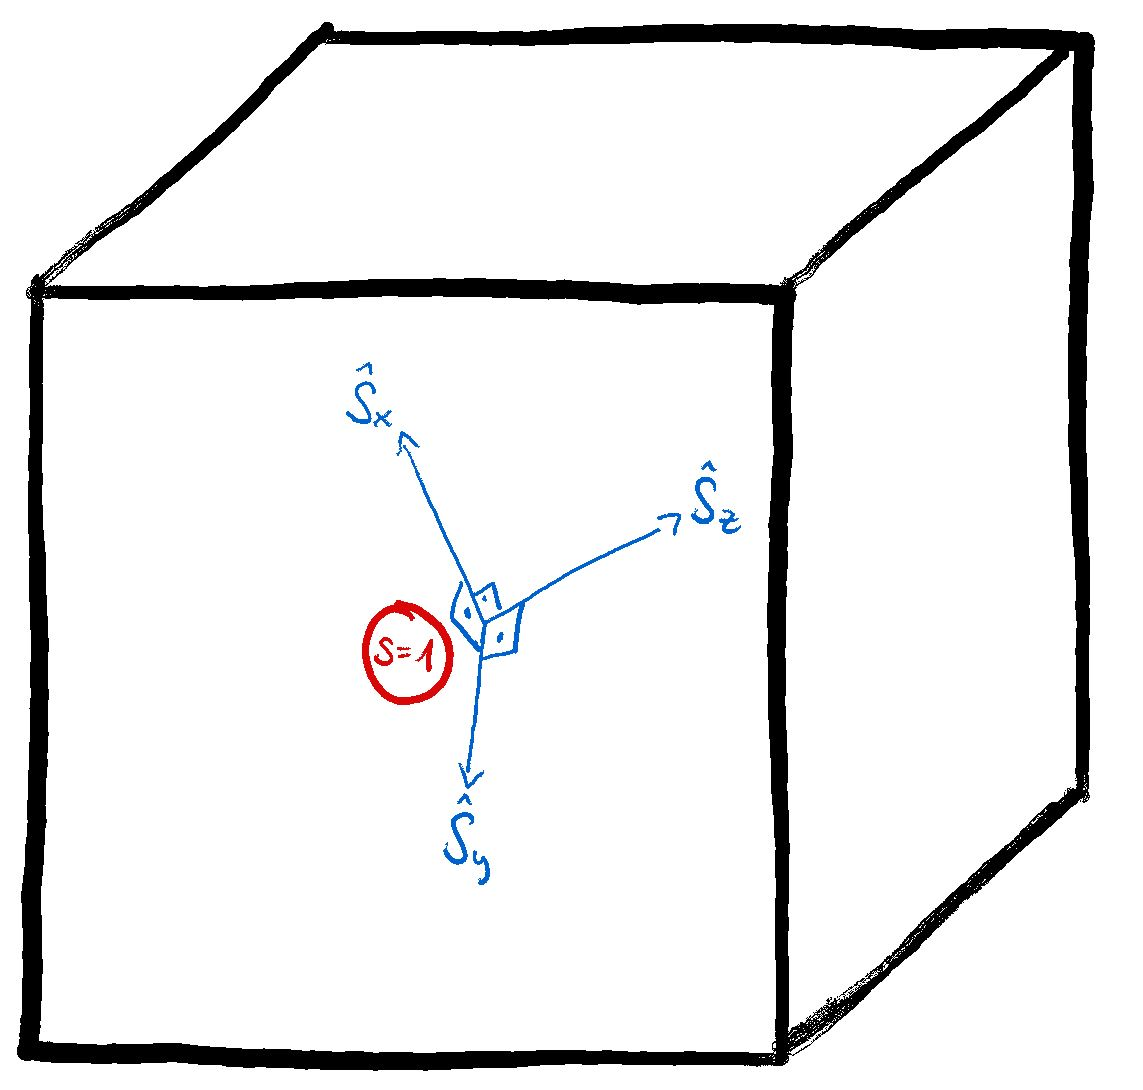
\includegraphics[width=0.8\textwidth]{box.jpg}
\end{flushright}
  \end{columns}
\end{frame}
\subsection{A na\" ive measurement process}
\begin{frame}{ }
\begin{itemize}
\item $\hat S_i,\hat S_j, i\neq j$ not compatible observables
\item $\left\{\hat S_i^2\right\}_{i\in\{x,y,z\}}$ are compatible observables\\
\textit{Proof:}
\begin{align*}
[\hat S^2_i,\hat S^2_j]&=\hat S_i\hat S_j[\hat S_i,\hat S_j]+\hat S_i[\hat S_i,\hat S_j]\hat S_j+\hat S_j [\hat S_i,\hat S_j]\hat S_i+ [\hat S_i,\hat S_j]\hat S_j\hat S_i\\ \quad& 
=i(\underbrace{\hat S_i\hat S_j\varepsilon_{ijk}\hat S_k+\hat S_i\varepsilon_{ijk}\hat S_k\hat S_j}_{=0 (j\leftrightarrow k)}+\underbrace{\hat S_j \varepsilon_{ijk}\hat S_k\hat S_i+\varepsilon_{ijk}\hat S_k\hat S_j\hat S_i}_{=0 (j\leftrightarrow k)}) \\ \quad& =0
\end{align*}
\item measure $\hat S_i^2$ along any given axis
\item $\hat S_i^2$ has two eigenvalues $s^2_i=0,1$ for $ i\in\{x,y,z\}$
\item $\hat S_x^2+\hat S_y^2+\hat S_z^2=s(s+1)|_{s=1}=2$
\end{itemize}
$\Rightarrow$ measuring the squared spin components in three perpendicular directions yields (101) and permutations thereof
\end{frame}
\begin{frame}
BUT:
\begin{block}{Consequence of Kochen-Specker Theorem}
    The measurement outcome CANNOT be the result from detecting (hypothetically) predetermined values of the squared spin components
  \end{block}
Definition 101-function (cp. \cite{conway2008strong}):
\begin{enumerate}
\item assigns measurement outcome to an axis
\item Opposite directions give the same answer for measuring the squared spin components.
\item Two perpendicular directions cannot both be 0.
\item Three perpendicular directions cannot all be 1.
\end{enumerate}
We will see:
\begin{block}{Kochen-Specker Theorem (our early version)}
    $\nexists$ 101-function for arbitrary directions
  \end{block}
\end{frame}


\subsection{Creating a contradiction}

\begin{frame}{Proof of the KS Theorem}
\framesubtitle{(following \cite{conway2008strong} and \cite{Peres_1991})}
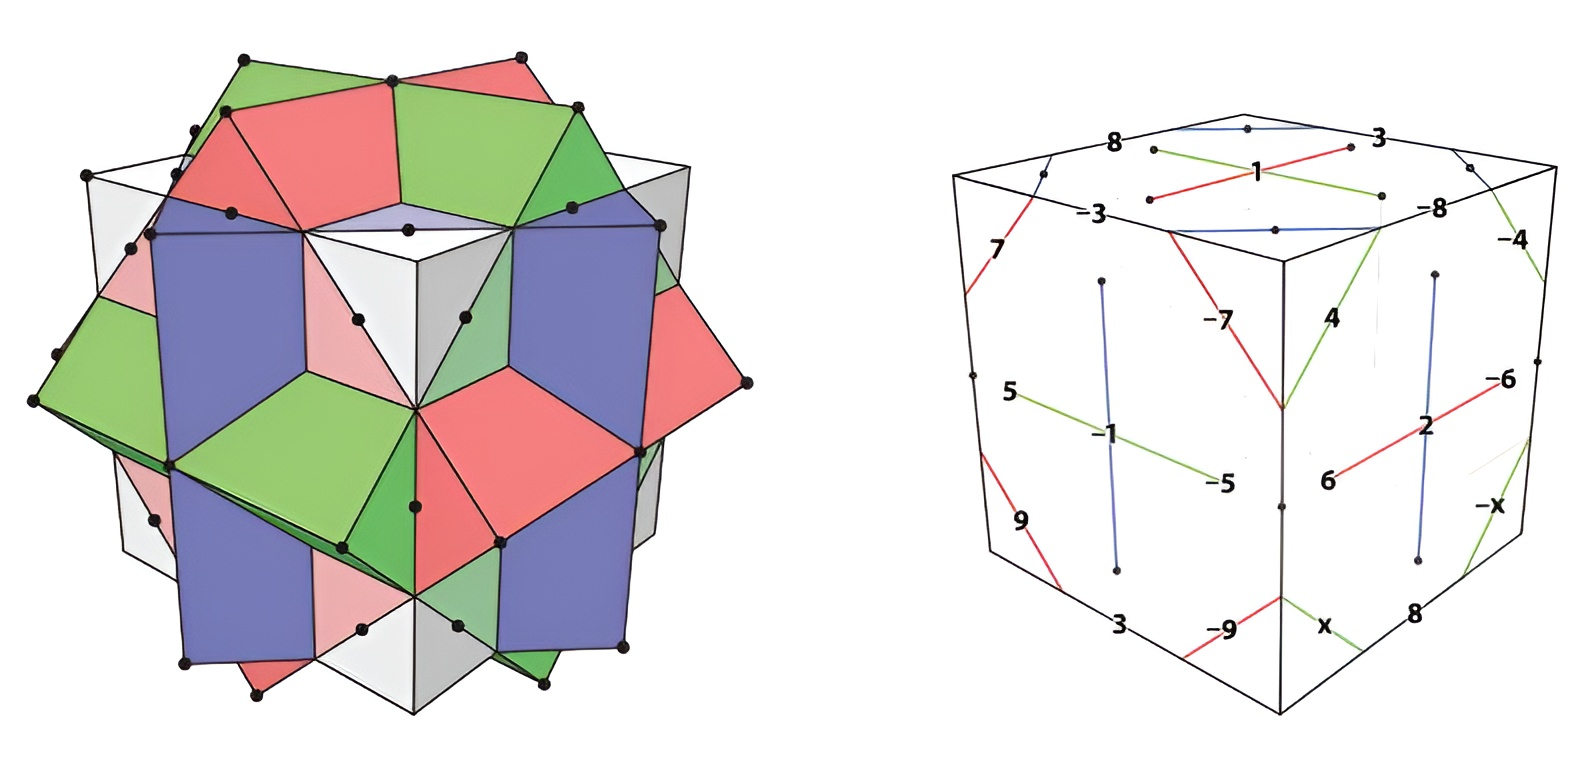
\includegraphics[width=\textwidth]{KSProof00.jpg}
\begin{tiny}
\begin{flushright}images from \cite{conway2008strong}, p. 3, upscaled\end{flushright}\end{tiny}
\end{frame}

\begin{frame}
\begin{itemize}
\item star node: 101-function takes value 1 on it; circle node: 101-function takes value 0 on it
\item axis defined by point goes to center of cube, each coordinate triple $(a,b,c)$ we are interested in defines three orthogonal axes. 
\item $(1,-1,2)$ is orthogonal triple, w.l.o.g. assign circle to 2
\end{itemize}
\begin{center}
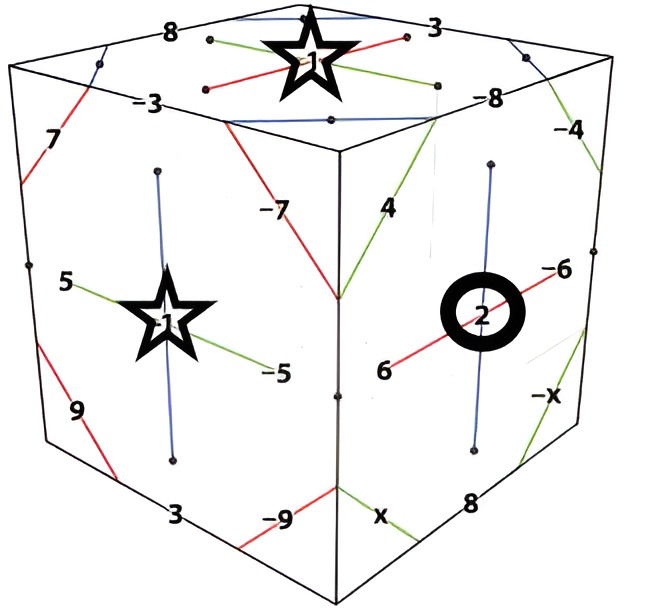
\includegraphics[width=0.5\textwidth]{KSProof01.jpg}
\end{center}
\end{frame}

\begin{frame}
\begin{itemize}
\item $(2,3,-3)$ is orthogonal triple $\Rightarrow\pm3$ star
\end{itemize}
\begin{center}
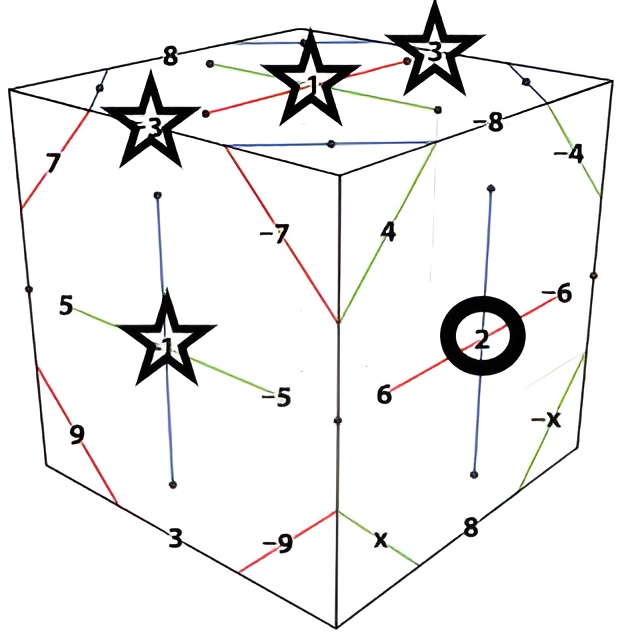
\includegraphics[width=0.5\textwidth]{KSProof02.jpg}
\end{center}
\end{frame}

\begin{frame}
\begin{itemize}
\item $(4,-x,3)$ is orthogonal triple 
\item w.l.o.g. 4 is circle (proof can proceed analogously if we say -4 is circle)
\end{itemize}
\begin{center}
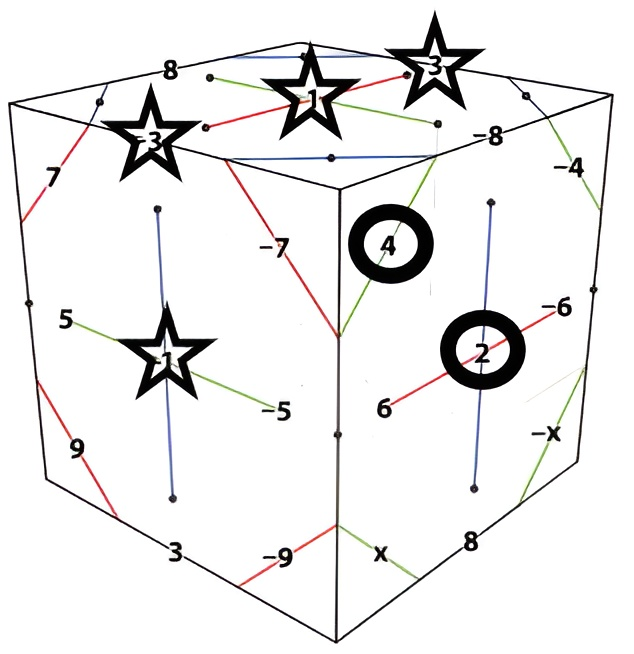
\includegraphics[width=0.5\textwidth]{KSProof03.jpg}
\end{center}
\end{frame}

\begin{frame}
\begin{itemize}
\item $(-4,x,-3)$ fixes that either -4 OR x is circle because -3 is star
\item if -4 is star: reflect around yellow plane \\ $\rightarrow$ -4 and x are interchanged every other circle or star node is left invariant\\
$\Rightarrow$ we may set -4 to circle
\end{itemize}
\begin{center}
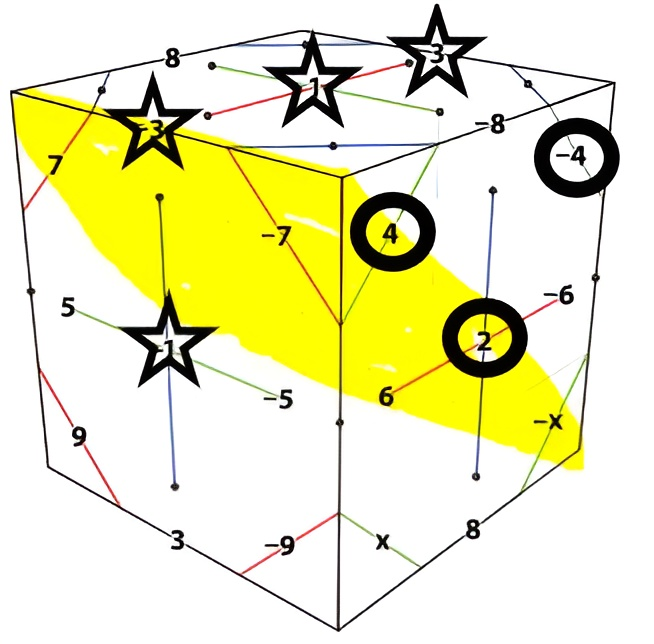
\includegraphics[width=0.5\textwidth]{KSProof04.jpg}
\end{center}
\end{frame}

\begin{frame}
\begin{itemize}
\item 5 is orth. to 4 $\Rightarrow$ 5 star
\item $(1,5,6)$ is orth. triple $\Rightarrow$ 6 circle
\item $(6,7,9)$ is orth. triple $\Rightarrow$ 7 and 9 star
\end{itemize}
\begin{center}
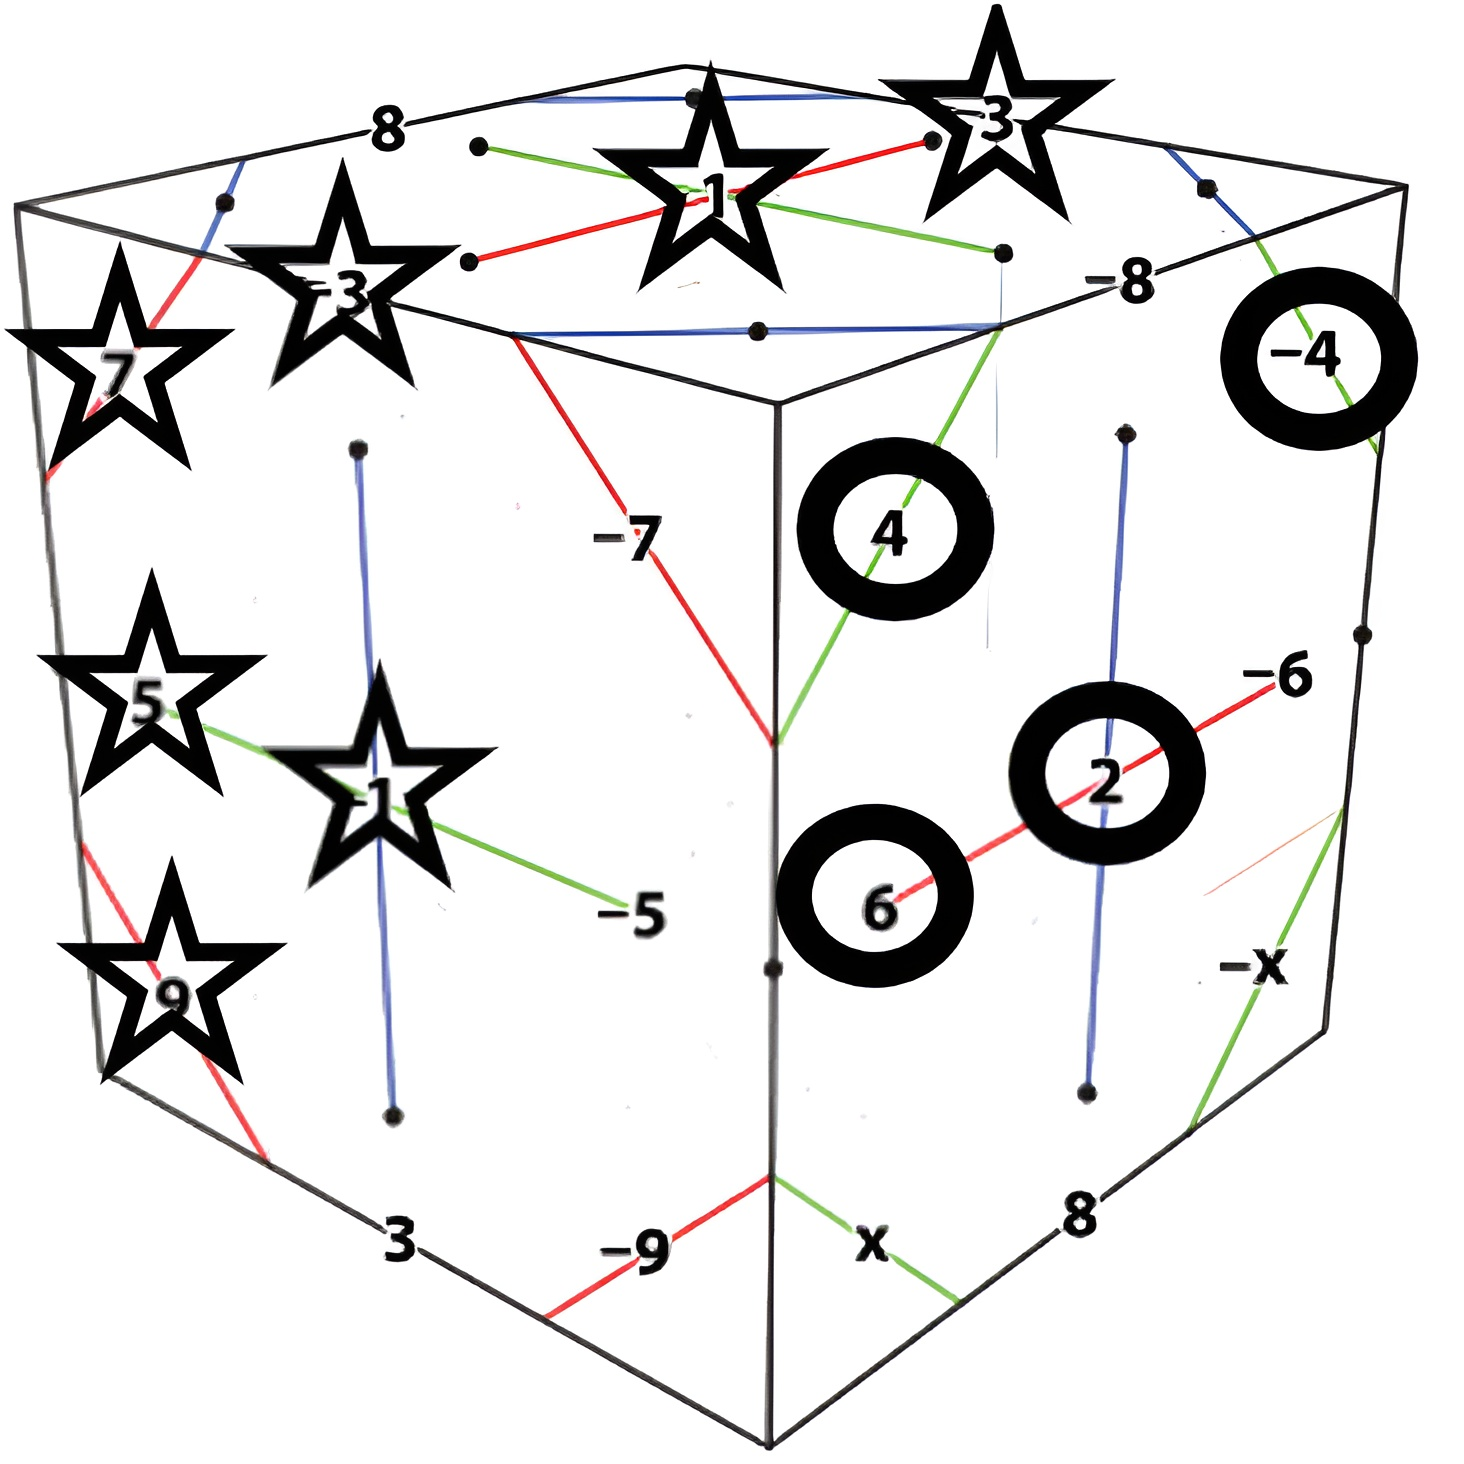
\includegraphics[width=0.5\textwidth]{KSProof05.jpg}
\end{center}
\end{frame}

\begin{frame}
\begin{itemize}
\item -5 is orth. to -4 $\Rightarrow$ -5 star
\item $(1,-5,-6)$ is orth. triple $\Rightarrow$ -6 circle
\item $(-6,-7,-9)$ is orth. triple $\Rightarrow$ -7 and -9 star
\end{itemize}
\begin{center}
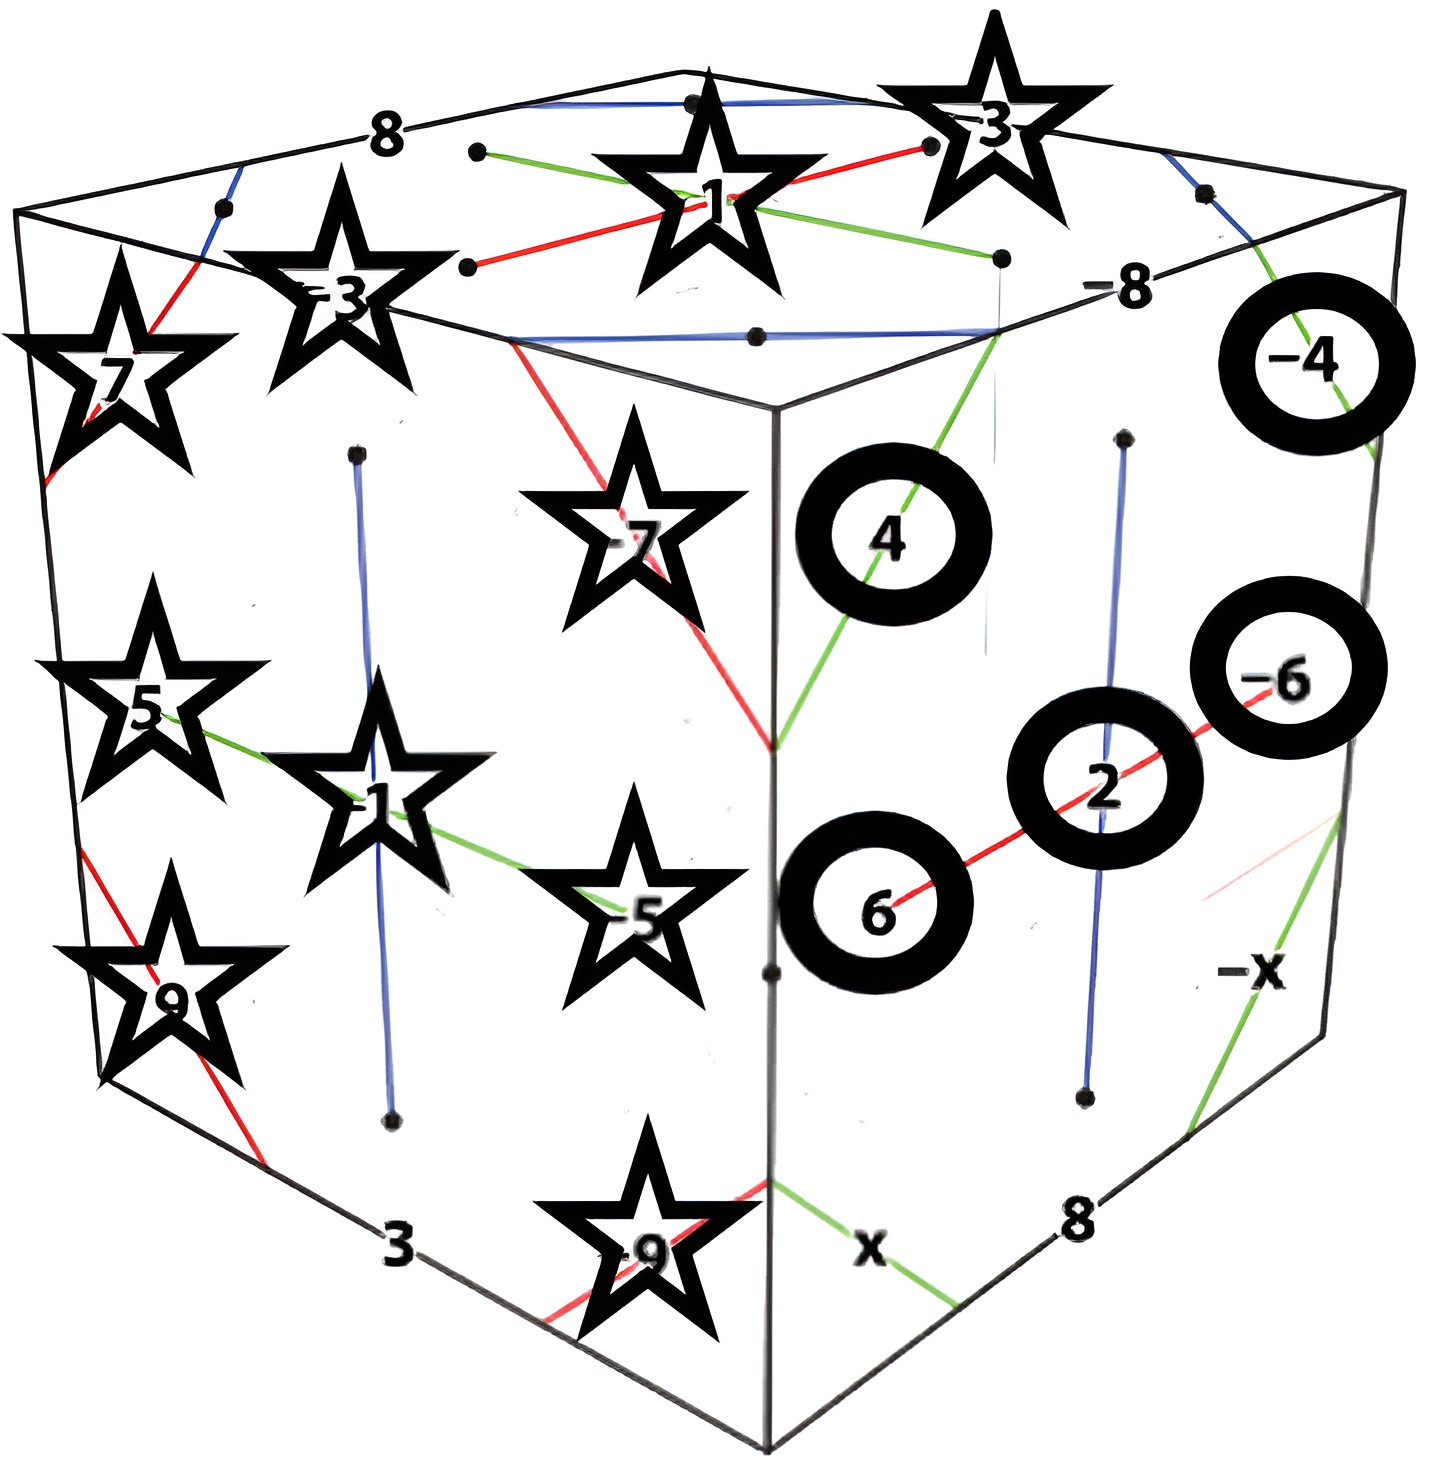
\includegraphics[width=0.5\textwidth]{KSProof06.jpg}
\end{center}
\end{frame}

\begin{frame}
\begin{itemize}
\item $(8,-7,9)$ is orth. triple $\Rightarrow$ 8 has to be circle
\item $(-8,7,9)$ is orth. triple $\Rightarrow$ -8 has to be circle
\item BUT: 8 is orthogonal to -8  $\Rightarrow\lightning$
\end{itemize}
\begin{center}
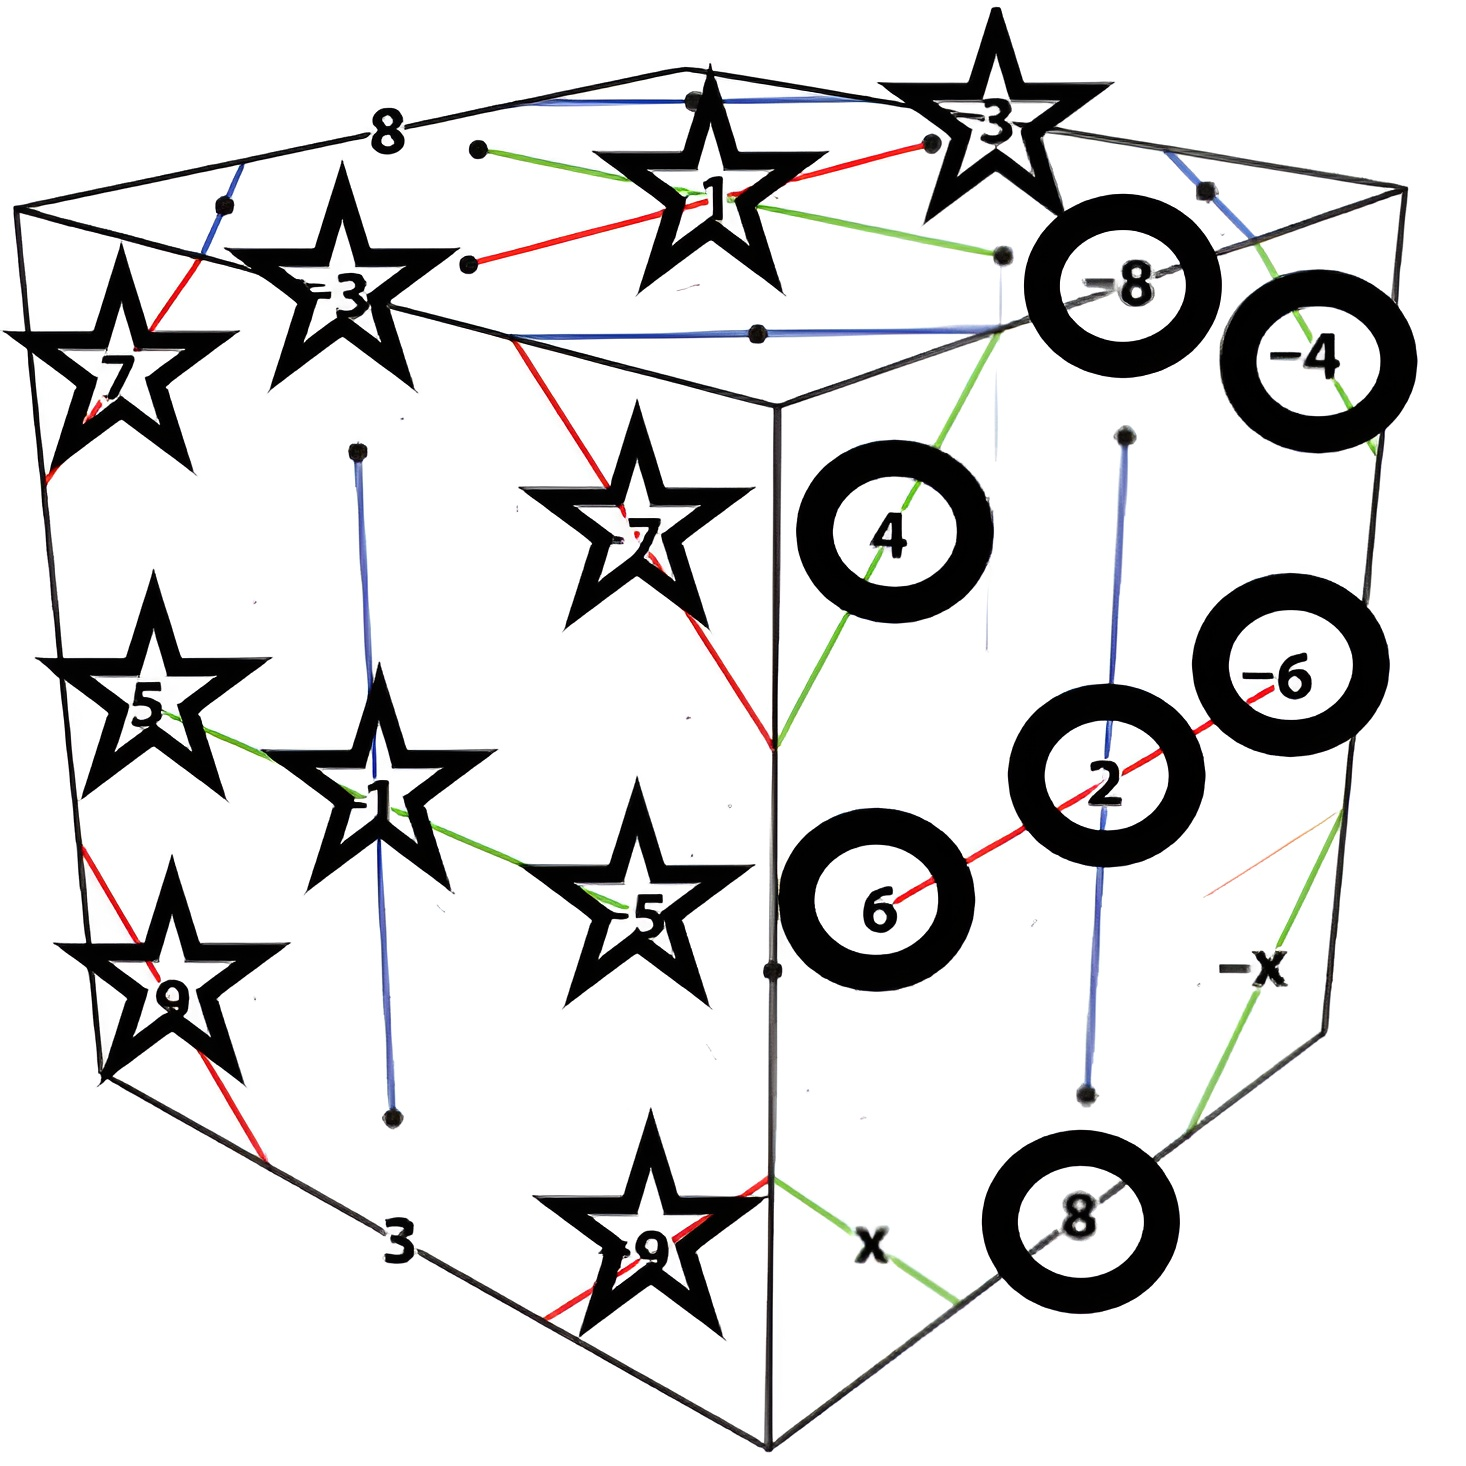
\includegraphics[width=0.5\textwidth]{KSProof07.jpg}
\end{center}
\end{frame}

\section{Tracing the origin of the contradiction}
\subsection{What assumptions were (secretly) made?}
\begin{frame}{What assumptions were (secretly) made?}
\begin{columns}
 \column{.05\textwidth}
    \column{.95\textwidth}
\begin{enumerate}
\item [(NA1)] The squared spin components are well defined for arbitrary orthogonal axes
\item [(NA2)] (measurement) value of the sum of the squared spin components = Sum of the (measurement) values of the squared spin components
\item [(NA3)] (measurement) value of the squared spin component = Square of the (measurement) value of the spin component
\end{enumerate}
\end{columns}
\vfill
These lead directly to...
\end{frame}

\subsection{The Kochen-Specker Theorem in full strength}
\begin{frame}{The Kochen-Specker Theorem}
\framesubtitle{(our semi-final version, cited from \cite{sep-kochen-specker})}
\begin{block}{KS Theorem}
Let $\mathcal{H}$ be a Hilbert space of QM state vectors of dimension $x\geq3$. There is a set $\mathcal M$ of observables on $\mathcal{H}$, containing $y$ elements, such that the following two assumptions are contradictory: 
  \begin{columns}
    \column{.05\textwidth}
    \column{.95\textwidth}
\begin{itemize}
\item [(KS1)] All $y$ members of $\mathcal M$ simultaneously have values, i.e. are unambiguously mapped onto real numbers (designated, for observables $A,B,C,...\in\mathcal M$ by $\nu(A),\nu(B),\nu(C),...\in\mathbb{R}$
\item [(KS2)] Values of all observables in $\mathcal M$ conform to the following constraints:
\begin{itemize}
\item [(a)] $A,B,C\in\mathcal M$ pairwise compatible with $C=A+B\Rightarrow \nu(C)=\nu(A)+\nu(B)$
\item[(b)] $A,B,C\in\mathcal M$ pairwise compatible with $C=A\cdot B\Rightarrow \nu(C)=\nu(A)\cdot\nu(B)$
\end{itemize}
\end{itemize}
  \end{columns}

\end{block}
\end{frame}
\begin{frame}
Remarks:
\begin{itemize}
\item There is no such statement for $\mathrm{dim}\mathcal H=x<3$
\item If proven for $x=3$, the theorem follows for $\mathrm{dim}\mathcal H>3$ because $\mathcal H$ has at least one subspace of dimension three in which the statement holds. %This assumes (O) $\rightarrow$ next slide
\item If we do not assume a correspondence between operators on $\mathcal H$ and observables in $\mathcal M$, (KS2) could be understood as a definition of the addition and multiplication of observables.
\item (KS2)$\Rightarrow$(NA2) and (KS2)$\Rightarrow$(NA3)
\item (KS1)$\Rightarrow$(NA1)
\end{itemize}
\vfill
\begin{center}
$\Rightarrow$ The non-existence of 101-functions proves the KS Theorem in full strength.
\end{center}
\end{frame}

\begin{frame}
%\begin{columns}
 %\column{.05\textwidth}
   % \column{.95\textwidth}
%\begin{enumerate}
%\item [(O)] There is a one-one correspondence between properties of a quantum system and projection operators on the system’s Hilbert space
%\end{enumerate}
%\end{columns}
%\vspace{10pt}

For future reference:
\begin{columns}
 \column{.05\textwidth}
    \column{.95\textwidth}
\begin{enumerate}
\item [(VD)] All observables defined for a QM system have definite values at all times.
\end{enumerate}
\end{columns}
\vspace{10pt}
Obviously (KS1)$\iff$ (VD)
\vfill
For the term 'measurement' to be well-defined in the way we used it before we need another assumption:
\begin{columns}
 \column{.05\textwidth}
    \column{.95\textwidth}
\begin{enumerate}
\item [(NC)] If a QM system possesses a property (value of an observable), then it does so independently of any measurement context, i.e. independently of \textit{how} that value is eventually measured. 
\end{enumerate}
\end{columns}
\end{frame}

%The key ingredients of the KS theorem are the constraints on value assignments spelled out in (2): the Sum Rule and Product Rule. They can be derived from a more general principle, called the Functional Composition Principle (FUNC)

\section{The FUNC Principle}
\subsection{Valuation Functions} %(and the FUNC principle)
\begin{frame}{Valuation Functions in Classical Theory}
\framesubtitle{(following \cite{topos})}
\begin{block}{Physical quantities}
Any physical quantity $A$ is represented by function from the state space $S$ to the reals $$f_A:S\rightarrow\mathbb R$$
We call $f_A(s_i)$ the value of $A$ for a state $s_i\in S$.
\end{block}
Remark:
\begin{itemize}
\item Let $A$ be a physical quantity which is described by two distinct functions $f_A,f_A^\prime$ (from the state space to the reals). Then $\exists s\in S: f_A(s)\neq f^\prime_A(s)\Rightarrow$ the value of $A$ is not well-defined for a state $s\lightning$ to classical theory \\ $\Rightarrow$ for each $A$ there corresponds exactly one function $f_A$
\end{itemize}
\end{frame}

\begin{frame}
\begin{block}{Classical valuation functions}
$\forall s_i\in S$ define the valuation function $V_{s_i}$ as the function which assigns an observable $A$ from the set observables $\mathcal O$ the value of $A$ for the state:
$$
V_{s_i}:\mathcal O\rightarrow\mathbb R,\ A\mapsto V_{s_i}(A)\defeq f_A(s_i)
$$
\end{block}
\end{frame}

\begin{frame}{The functional composistion principle}
\framesubtitle{in classical theory}
\begin{block}{The classical FUNC principle}
For all functions $h:\R\rightarrow\R$, physical quantities $A\in\mathcal O$ and states  $s_i\in S$:
$$V_{s_i}(h(A))=h(V_{s_i}(A))$$
where $h(A)\defeq (h\circ f_A)$

\end{block}
\vfill
Example:\\
Let $h:\R\rightarrow\R, x\mapsto x^2$ and $A\defeq E$ be the energy of a state $s_i$. The classical FUNC principle now tells us: \textit{"the value of the energy squared is equal to the square of the value of the energy"} %seems quiet plausible, because why would nature care wether I measure the energy and square it afterwards or whether I measure the square of the energy directly. It is besides the point here how one would accomplish such a measurement
\end{frame}

\begin{frame}{Valuation Functions in Quantum Theory}
\begin{itemize}
\item if a state $|\psi\rangle$ is not an eigenstate of $A\in\mathcal O$, it makes not sense to extend the classical definition for valuation functions to quantum systems
\end{itemize}

\begin{block}{The quantum FUNC principle}
A valuation function for quantum theory is a map $V_{|\psi\rangle}:\mathcal O\rightarrow\R$ which satisfies the following two conditions:
\begin{itemize}
\item [$(i)$] $V_{|\psi\rangle}(\hat A)\in\sigma(\hat A)\subseteq\R$ represents the value of the operator $\hat A$ given a state $|\psi\rangle\in\mathcal H$. $\sigma(\hat A)$ is the spectrum of $\hat A\in\mathcal O$
\item [$(ii)$] FUNC: 
$$
V_{|\psi\rangle}(h(\hat A))=h(V_{|\psi\rangle}(\hat A))\ \forall h:\R\rightarrow\R
$$
\end{itemize}
\end{block}
\vfill
Remark:
\begin{itemize}
\item In some contexts it makes sense to define $V_{|\psi\rangle}:\mathcal O\rightarrow P([\R])$ where $P([\R])$ is the set of all probability distributions.
\end{itemize}
\end{frame}

\begin{frame}{What is meant by $h(\hat A)$?}
\begin{enumerate}
\item If $|\psi\rangle\in\mathcal H$ and $\hat A|\psi\rangle=a|\psi\rangle$ for some $a\in\R$:
$$
h(\hat A)|\psi\rangle\defeq h(a)|\psi\rangle
$$
\item $\hat A=\displaystyle\sum\limits_{a\in\sigma(\hat A)}a  \hat P_a\rightarrow  h(\hat A)\defeq\displaystyle\sum\limits_{a\in\sigma(\hat A)}h(a)  \hat P_a$\\ %\displaystyle\SumInt\limits_{\sigma(\hat A)}a \mathrm d \hat P_a$
\vfill
Remarks:
\begin{itemize}
\item [(a)] $\hat P_a$ is the projector on the eigenspace of eigenvalue $a\in\sigma(\hat A)$
\item [(b)] We assume discrete $\sigma(\hat A)$. Generalization for general $\sigma(\hat A)\subseteq\R$ possible, but not trivial ($\rightarrow$ \href{https://en.wikipedia.org/wiki/Projection-valued_measure}{Projection-valued measures})
\end{itemize}
\end{enumerate}
\end{frame}
\subsection{The STAT FUNC Principle}

\begin{frame}{The statistical functional composition principle}
\begin{block}{The STAT FUNC Principle}
Let $\hat A$ be a self-adjoint operator representing an observable $A$ and let $f:\R\rightarrow\R$ be a function. Then for all $a\in\R$:
$$
\mathrm{prob}\left[V_{|\psi\rangle}(f(\hat A))=a\right]=\mathrm{prob}\left[f(V_{|\psi\rangle}(\hat A))=a\right]
$$
\end{block}
\vfill
\begin{itemize}
\item Note that we do not require $(ii)$ from the definition of the quantum FUNC principle for our $V_{|\psi\rangle}$ here. %because then STAT FUNC would be trivial
\item Gleasons Theorem \cite{10.2307/24900629}: On a Hilbert space $\mathcal H$ with $\mathrm{dim}\mathcal H\geq 3$, the only probability measures are of the form
$$
\mu(\hat P_\alpha)\defeq\mathrm{Tr}\left(\hat P_\alpha\hat\rho\right)
$$
where $\hat P_\alpha$ is a projection operator and $\hat\rho$ is the operator which characterizes the system's state ("density matrix").\\
$$\Rightarrow\mathrm{prob}\left[V_{|\psi\rangle}(\hat A)=a\right]=\mathrm{Tr}(\hat P_{|a\rangle}\cdot\hat P_{|\psi\rangle})$$
\end{itemize}
\end{frame}

\begin{frame}[allowframebreaks]{Proving the STAT FUNC Principle}
\begin{itemize}
\item Characteristic function: $\chi_{r}: \R\rightarrow \{0,1\}, t\mapsto\chi_{r}(t)=\begin{cases} 1, r=t\\ 0, r\neq t  \end{cases}$
\item $\chi_r(\hat A)\defeq \displaystyle\sum\limits_{a\in\sigma(\hat A)}\chi_{r}(a)\hat P_a=\begin{cases} \hat P_r, r\in\sigma(\hat A)\\ 0, \mathrm{else}  \end{cases}$\\
$\Rightarrow\mathrm{prob}\left[V_{|\psi\rangle}(\hat A)=a\right]=\mathrm{Tr}(\hat P_{|a\rangle}\cdot\hat P_{|\psi\rangle})=\mathrm{Tr}(\chi_a(\hat A)\cdot\hat P_{|\psi\rangle})$
\item $\chi_r(f(\hat A))=\left.\begin{cases} \hat P_r, f(r)\in\sigma(f(\hat A))\\ 0, \mathrm{else}\end{cases}\right\}=\chi_{f^{-1}(r)}(\hat A)$ % because r in sigma(f(A)) iff f^(-1)(r) in sigma(A)
%\begin{cases} \hat P_{f^{-1}(r)}, f^{-1}(r)\in\sigma(\hat A)\\ 0, \mathrm{else}  \end{cases}$ 
\end{itemize}
\framebreak 
\begin{align*}
\mathrm{prob}\left[V_{|\psi\rangle}(f(\hat A))=a\right] &= \mathrm{Tr}\left( \chi_{f^{-1}(a)}(\hat A)\cdot \hat P_{|\psi\rangle}\right)\\ \quad&
										=  \mathrm{Tr}\left( \hat P_{f^{-1}(a)}\cdot \hat P_{|\psi\rangle}\right)\\ \quad&
										= \mathrm{prob}\left[V_{|\psi\rangle}(\hat A)=f^{-1}(a)\right] \\ \quad& 
										= \mathrm{prob}\left[f(V_{|\psi\rangle}(\hat A))=a\right]  \\ \quad& 
											&\hfill \square
\end{align*}	
\end{frame}
%\subsection{Proof of the STAT FUNC Principle}
\subsection{The FUNC Principle}
\begin{frame}[allowframebreaks]{The FUNC Principle: Proof}
\begin{block}{Value realism}
$\forall \alpha\in[0,1]$ and for all operators $\hat A$ s.t. $\alpha =\mathrm{prob}\left[V(\hat A)=\beta\in\R \right]$ there corresponds an observable $A$ with value $\beta$
\end{block}
$$
\begin{rcases}
\mathrm{(NC)}\\
\mathrm{(VD)}\\
\mathrm{(VR)}\\
\mathrm{STAT\ FUNC}
\end{rcases}\Rightarrow \mathrm{FUNC}
$$
\\
\framebreak
\textit{Proof:}\\
\begin{itemize}
\item Consider an observable B represented by the (self-adjoint) operator $\hat B$ and a state $|\psi\rangle$.
\item From (VD): $\exists b\in\R:\ V_{|\psi\rangle}(\hat B)=b$
\item For $f:\R\rightarrow\R$ we obtain $f(V_{|\psi\rangle}(\hat B))=f(b)\eqdef a\in\R$
\item From STAT FUNC: $\mathrm{prob}\left[f(V_{|\psi\rangle}(\hat B))=a\right]=\mathrm{prob}\left[f(V(_{|\psi\rangle}(\hat B))=a\right] \Rightarrow\exists$ self-adjoint $f(\hat B)$
\item From (VR): The observable which corresponds to $f(\hat B)$ exists and has value $a\Rightarrow f(V_{|\psi\rangle}(\hat B))=V_{|\psi\rangle}(f(\hat B))$. 
\item From (NC): $a$ is unique $\hfill\square$
\end{itemize}


%What is (VR)?


\end{frame}



\subsection{Consequences of the FUNC Principle}



\begin{frame}[allowframebreaks]{Consequences of the FUNC Principle}
The sum (KS2a) and product rule (KS2b) follow from FUNC:\\
\vfill
\textit{Proof of (KS2a):}

\begin{itemize}
\item From functional analysis: $\forall\hat A,\hat B$ compatible and $\exists f,g:\R\rightarrow\R,\hat C$ s.t. $\hat A=f(\hat C),\hat B=g(\hat C)$
\item Let $h\defeq f+g\Rightarrow \hat A+\hat B=h(\hat C)$
\item $V(\hat A+\hat B)=V(h(\hat C))=h(V(\hat C))=f(V(\hat C))+g(V(\hat C))=V(f(\hat C))+V(g(\hat C))=V(\hat A)+V(\hat B)$
\end{itemize}
\vfill
(KS2a) follows similiarly.\\
\framebreak
From the sum and product rule we immediately get:
\begin{itemize}
\item The identity operator has to take value 1
\item The zero operator has to take value 0
\item Projectors have to take either value 0 or 1
\end{itemize}
\framebreak
\begin{block}{Alternate form of KS Theorem}
Let $\mathcal{H}$ be a Hilbert space of QM state vectors of dimension $x\geq3$. There is a set $\mathcal M$ of observables on $\mathcal{H}$, containing $y$ elements, such that the following two assumptions are contradictory: 
  \begin{columns}
    \column{.05\textwidth}
    \column{.95\textwidth}
\begin{itemize}
\item [(KS1')] All $y$ members of $\mathcal M$ simultaneously have values, i.e. are unambiguously mapped onto real numbers (designated, for observables $A,B,C,...\in\mathcal M$ by $\nu(A),\nu(B),\nu(C),...\in\mathbb{R}$.
\item [(KS2')] Values of all observables obey the FUNC principle.
\end{itemize}
  \end{columns}
\end{block}
\end{frame}
\section{Consequences of KS Theorem}
\begin{frame}{Consequences of KS Theorem}
If our reasoning to this point was correct (i.e. the axioms of QM themselves are flawed!), (KS1$^{(')}$) or (KS2$^{(')}$) has to be incorrect.
\vfill
{\Huge
\begin{center}
$\rightsquigarrow$ John :)
\end{center}
}

\end{frame}


%\section{Alternative approaches to proving the KS Theorem}




%\nocite{*}
%\phantomsection\addcontentsline{toc}{chapter}{Bibliography}
\begin{frame}[allowframebreaks]{Bibliography}
\printbibliography
\end{frame}

\end{document}
